\documentclass[a4paper]{article}

\pdfmajorversion=1
\pdfminorversion=7
\pdfcompresslevel=9
\pdfobjcompresslevel=2

\usepackage[hidelinks]{hyperref}
\usepackage[margin=60pt]{geometry}
\usepackage[utf8]{inputenc}
\usepackage[english]{babel}
\usepackage{graphicx}

\setlength{\parindent}{0pt}

\hypersetup{
    pdftitle={Formal Digital Twin of a LEGO® MINDSTROMS™ Production Plant},
    pdfauthor={Andrea Infantino, Riccardo Motta and Matteo Negro}
}

\newcommand{\figureref}[1]{Figure \ref{#1}}
\newcommand{\reference}[1]{\ref{#1}: \nameref{#1} (page \pageref{#1})}

\newcommand{\nbvspace}[1][3]{\vspace*{\stretch{#1}}}

\begin{document}

    \begin{titlepage}

        \begin{center}

            \nbvspace[1]

            
\includegraphics[width=0.3\columnwidth]{./images/polimi}

            \nbvspace[2]

            {\huge \textbf{\textsc{Formal Digital Twin of a LEGO® MINDSTROMS™ Production Plant}}} \\
            [3em]
            {\Large Formal Methods for Concurrent and Real-Time Systems} \\
            [1.5em]
            {\Large A.Y. 2022-2023}

            \nbvspace[8]

            \begin{tabular}{lrp{0.04\columnwidth}lrp{0.04\columnwidth}lr}
                \multicolumn{2}{c}{\Large \textbf{Andrea Infantino}} & & \multicolumn{2}{c}{\Large \textbf{Riccardo Motta}} & & \multicolumn{2}{c}{\Large \textbf{Matteo Negro}} \\
                Person ID & ??? & & Person ID & 10658639 & & Person ID & 10642961 \\
                Student ID & ??? & & Student ID & 218685 & & Student ID & ???
            \end{tabular}

            \nbvspace[1]

        \end{center}

    \end{titlepage}

    \tableofcontents{}

    \pagebreak

    \section{Model Description}

    This section provides a description of the production plant with some implementation details, together with all the components that make it up. The motivations behind these modelling choices can be found in Section \reference{section:design_decisions}.

    \subsection{The Production Plant}

    \begin{figure}[h!]
        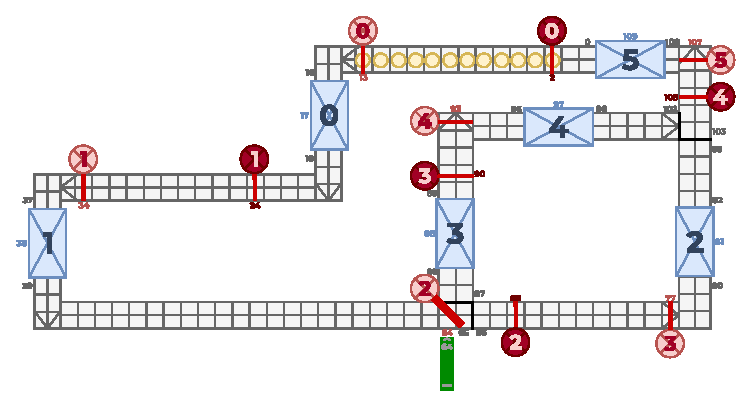
\includegraphics[width=\columnwidth]{./images/plant}
        \caption{the production plant we modelled.}
        \label{figure:scheme}
    \end{figure}

    \paragraph{Differences with the original} This model presents some differences with respect to the one presented in class. First, the position of what we refer to as the \textit{Flow Controller} has been moved from position 64 to position 65 in order to make it more consistent with the scheme of the plant and to avoid overlaps with the sensor already present at position 64, and second, position 107 was previously divided in two different slots, but since one of the two was so small that was barely visible, we decided to merge them into a single one.

    \paragraph{Notes on the scheme} We enhanced the original scheme with the number the various stations and laser sensors have inside our project and with the numbers of the positions of the conveyor belt, in order to respect what we have done inside the project.

    \subsection{General Overview}

    The model of our system is made of 6 different components which interact between them in order to coordinate the entire production plant. Some of them are also instantiated many times in order to have a simpler modelling of the entire system.

    \paragraph{Initializer} It's a fictitious component which represents the entry point of the whole system. It allows us to instantiate all the workpieces in the correct positions of the conveyor belt (positions which start from position 13 and ends in position 2 in our model) and works ad the motor, allowing the whole system to move synchronously.

    \paragraph{Conveyor belt} It's the set of all the various conveyor belts of the plant. It's the one in charge of moving around all the workpieces. In our model it's also the one in charge of blocking pieces and stations from proceeding according to the pieces of information gathered by the laser sensors and the stations and also manages the positions where the two branches of the plant start and merge.

    \paragraph{Stations} They are the ones in charge of processing the various workpieces one they get into them. We have a single template for them which is instantiated as many times as needed in order to recreate the plant. They have all a position on the conveyor belt which is managed in a special way.

    \paragraph{Laser sensors} We have modelled them in two different ways according to their functionalities. The ones guarding the entrance of a station are called \texttt{InSensor}, while the ones guarding the queue and preventing the station right before it to release a workpiece are called \texttt{OutSensor}. Like the stations, they are represented as a single template (one for each type) instantiated multiple times.

    \paragraph{Flow controller} This is the green piece of \figureref{figure:scheme}. It is pre-configured with a specific policy (which is customizable) and decides whether to send the pieces once they get at position 65 of the conveyor belt. The available policies are the following ones:
    \begin{enumerate}
        \item[0.] % TODO: description of policy 0
        \item[1.] % TODO: description of policy 1
        \item[2.] % TODO: description of policy 2
        \item[3.] % TODO: description of policy 3
    \end{enumerate}

    \subsection{Components Description}

    \section{Design Decisions} \label{section:design_decisions}

    \section{Scenarios}

    \section{Conclusions}

\end{document}
